\begin{center}
    \vspace*{1.5cm}
    {\fontsize{20}{20}\textbf{\fontspec{Lucida Sans Unicode}E-sektionens visor}}\\
    \vspace{0.7cm}
    {\fontsize{12}{12}\textit{Om E:aren själv får välja}}  
\end{center}
\addtocwithheader{E-sektionens visor}  % Add entry to TOC and set header
\noBackground

\newpage
% \resetBackground

\begin{textblock*}{3cm}(4.9cm,7.6cm) % {width}(x, y)
    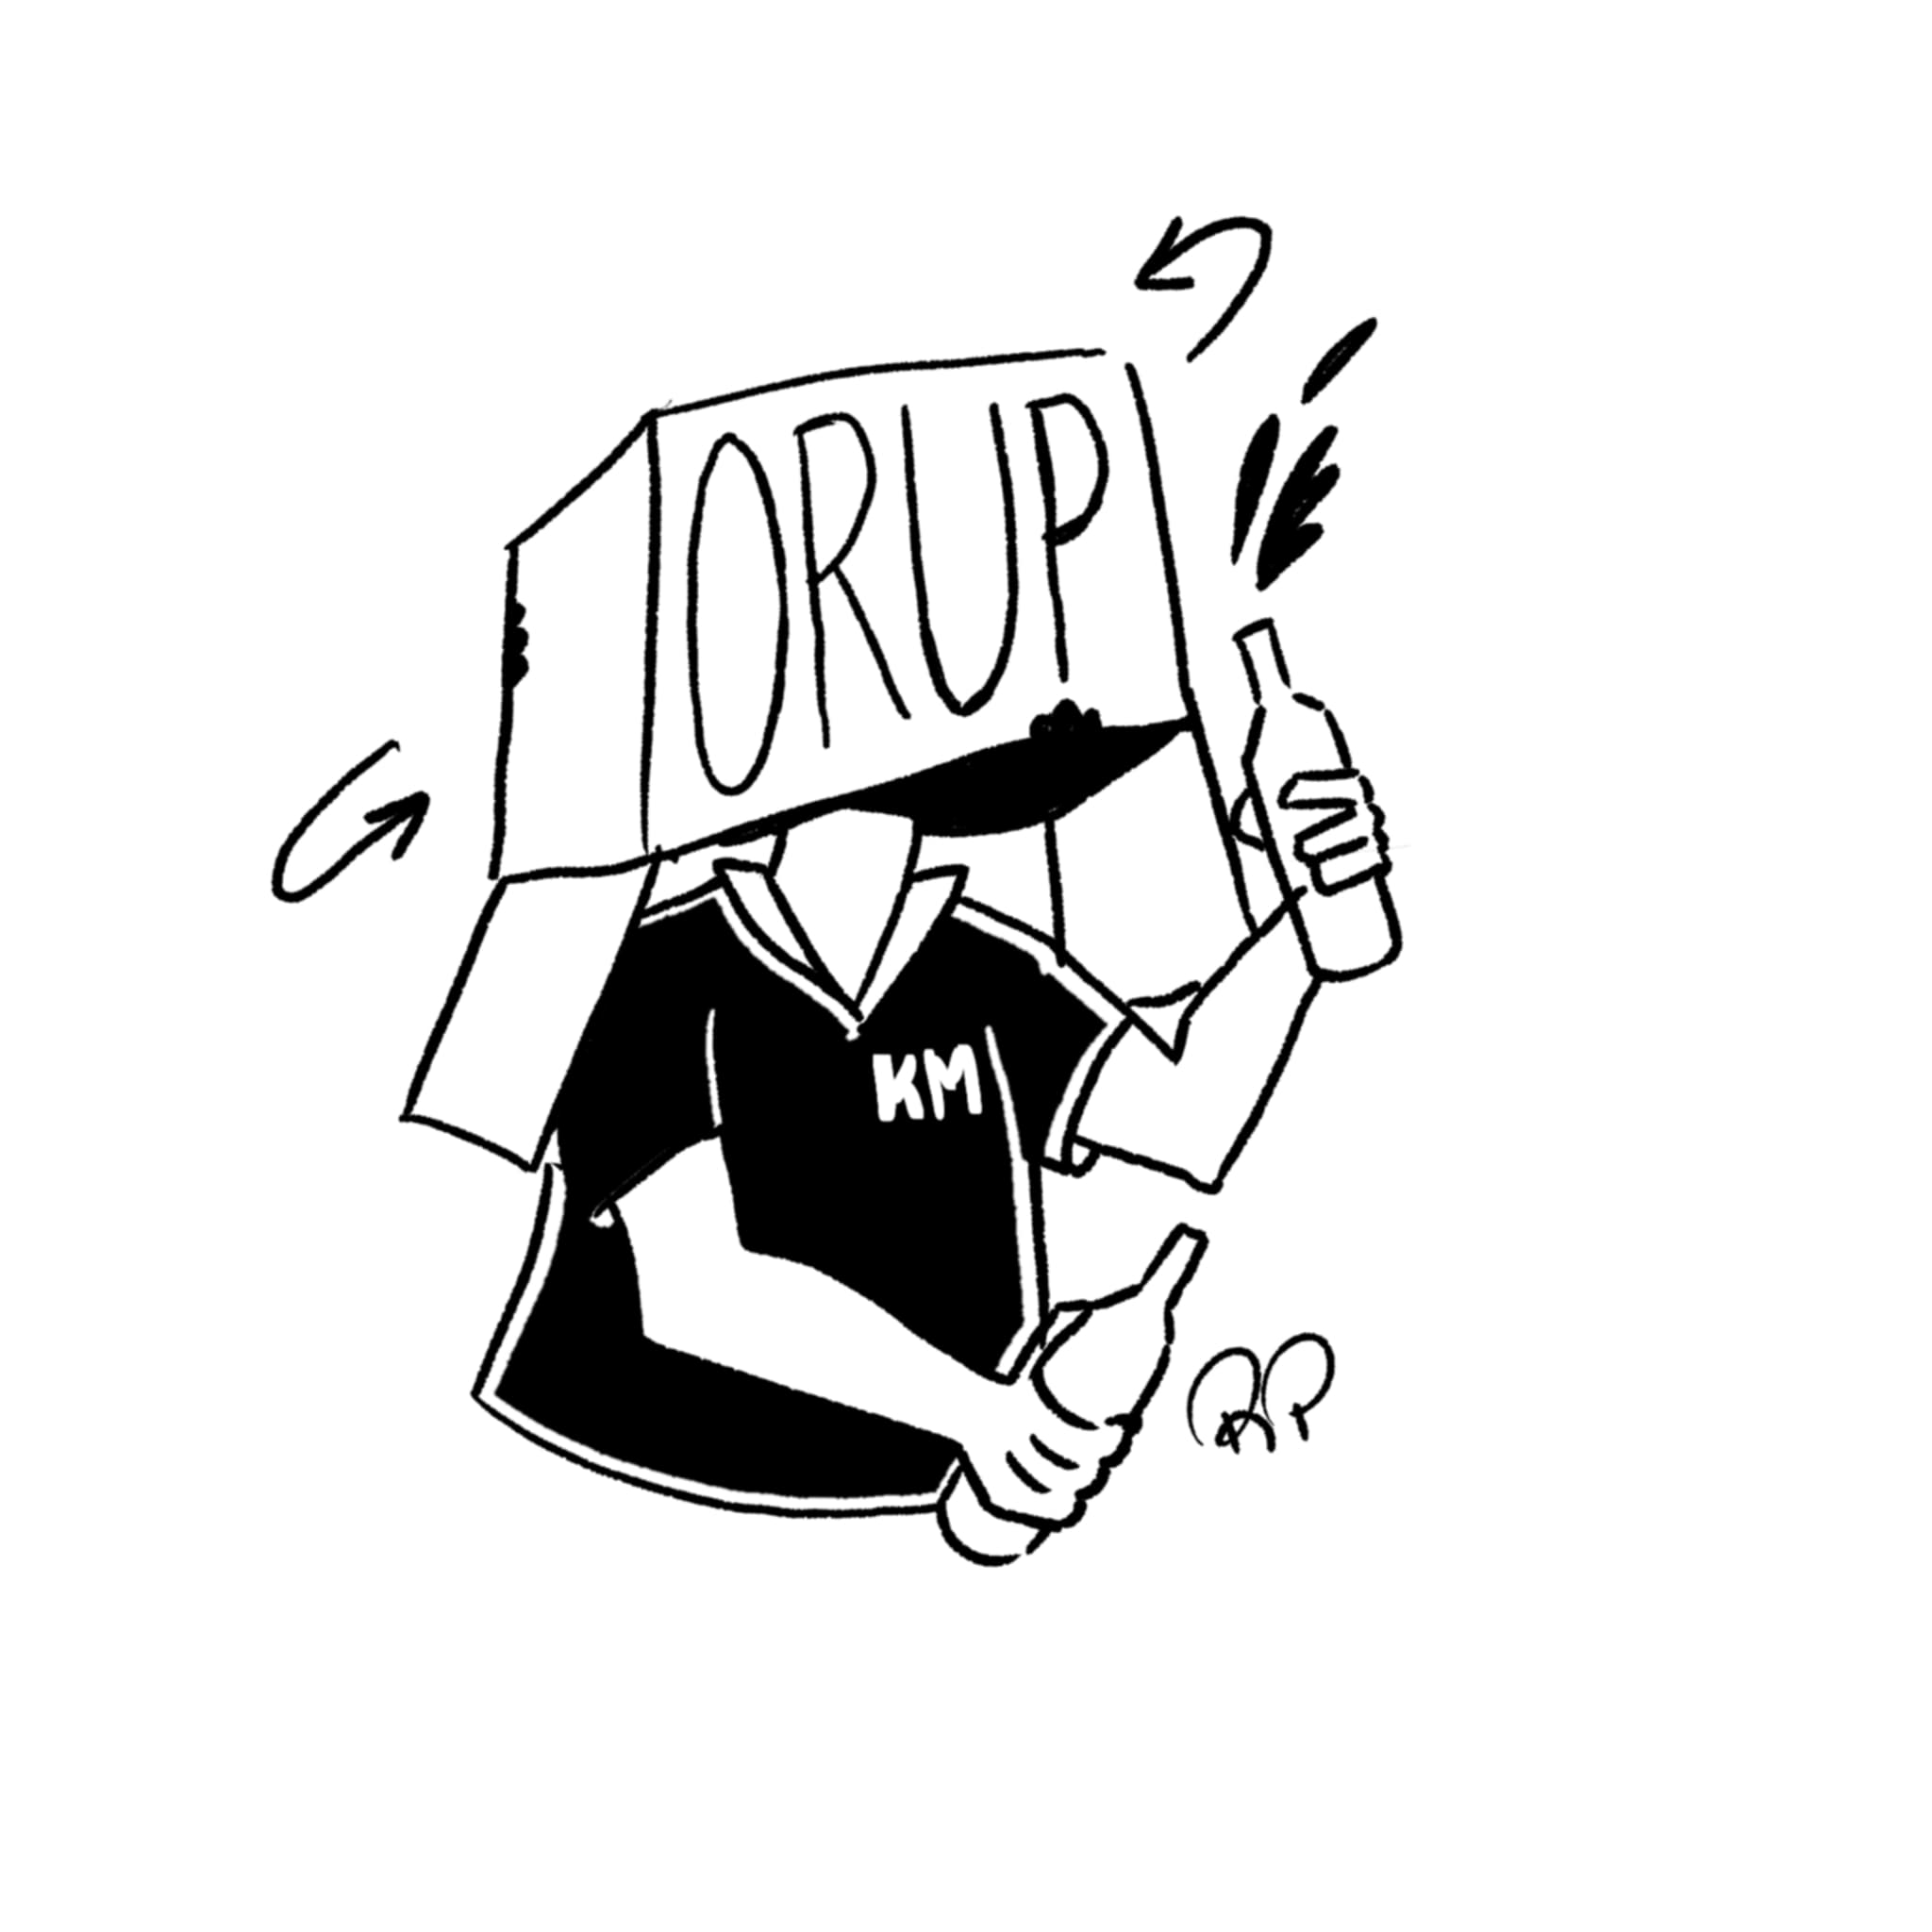
\includegraphics[width=6.0cm]{./bilder/ruths-bilder/orup.png}
\end{textblock*}

\subsection*{E-sektionens Kampvisa I}
\index[alfa]{E-sektionens Kampvisa I}
\index[anfa]{Det sprakar så glatt i vårt hår}
\songinfo{Mel: The Stars and Stripes Forever}

\begin{parse lines}[\noindent]{#1\\}
    Det sprakar så glatt i vårt hår
    ur öronen sprutar det gnistor
    och strömmarna i våra tår
    laddar upp oss när vi går

    I hjärnan vi har resistans
    och ström genom motstånd ger en spänning
    och spänning det vill vi ju ha
    Vi går på E! Vi går på E!
    Vi går på Elström!

\end{parse lines}


\subsection*{E-sektionens Kampvisa II} 
\index[alfa]{E-sektionens Kampvisa II}
\index[anfa]{E, E, E vill vi se}
\songinfo{Mel: Trink, trink, brüderlein trink}

\begin{parse lines}[\noindent]{#1\\}
    E, E, E vill vi se
    E är det bästa där é
    E, E, E vill vi se
    E får oss alla att le!
    Spänning där é i vår erotik
    vi kör med medicin och teknik
    Spänning där é i vår erotik
    vi kör med elektroteknik

\end{parse lines}

\vissteduatt{Visste du att Kampvisa II reviderades för att innefatta båda 
\\utbildningarna på E-sektionen?}

\newpage


\subsection*{E-sektionens Kampvisa III} 
\index[alfa]{E-sektionens Kampvisa III}
\index[anfa]{Vi é elteknister ifrån LTH}
\songinfo{Mel: Vi äro musikanter}

\begin{parse lines}[\noindent]{#1\\}
    Vi é elteknister ifrån LTH
    Hos oss finns inga brister och dé é ju som så

    (Att) Vi kan löda, räkna, dricka, bränna sprit
    Upp till Lophtet, kom så går vi dit!

    Vi kan räkna tangens, sinus, derivera, integraler
    Vi kan koda singelchip och mata våran pic

    Ett in, noll ut, rulla kabel, heja vit!
    Vi vill att just du skall komma hit

    Hoppa i din vita overall och börja gå
    Elteknik på LTH det bästa du kan få!

\end{parse lines}


\subsection*{E-sektionens Kampvisa IV} 
\index[alfa]{E-sektionens Kampvisa IV}
\index[anfa]{Vi vill ha mera E}
\songinfo{Mel: Mera mål}

\begin{parse lines}[\noindent]{#1\\}
    Vi vill ha mera E, flera E
    Å E det kommer ni att se
    Vi vill ha mera E, mycket mer
    Se upp här kommer vi från E

\end{parse lines}

\vissteduatt{Visste du att E-sektionen är den äldsta sektionen på LTH?}

\newpage


\subsection*{E-sektionens Kampvisa V} 
\index[alfa]{E-sektionens Kampvisa V}
\index[anfa]{Alla vi på E-sek klappar nu}
\songinfo{Mel: Klappa händerna}

\begin{parse lines}[\noindent]{#1\\}
    ||: Alla vi som går på E-sek klappar nu :||

\end{parse lines}


\subsection*{E-sektionens Kampvisa VI} 
\index[alfa]{E-sektionens Kampvisa VI}
\index[anfa]{Vi går på E-sek}
\songinfo{Mel: Man ska ha husvagn}

\begin{parse lines}[\noindent]{#1\\}
    Vi går på E-sek, och vi har spänning så som få
    Vi går på E-sek, äldst och bäst på LTH
    Vi går på E-sek, vår färg är vit, Elektrovit!
    Vi går på E-sek, LTH:s elit!

\end{parse lines}


\begin{textblock*}{3cm}(3.0cm,8.9cm) % {width}(x, y)
    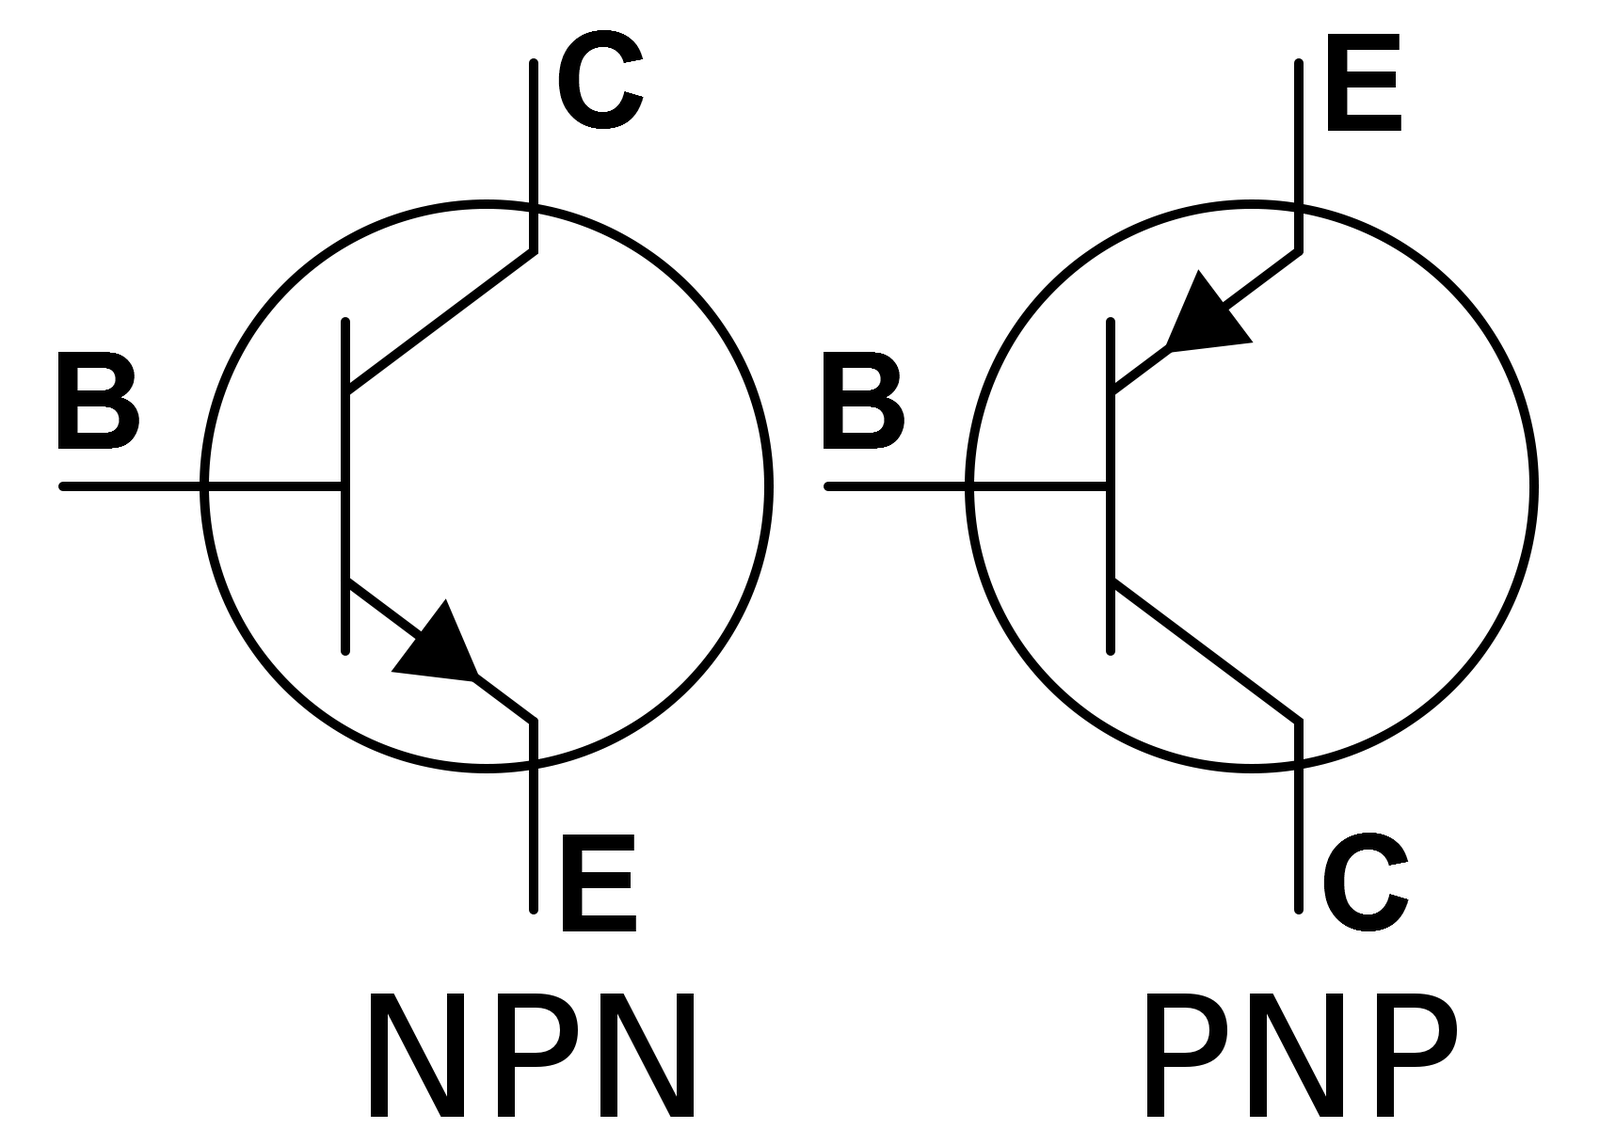
\includegraphics[width=4.5cm]{./bilder/Transistorer.png}
\end{textblock*}

\vissteduatt{Visste du att några kampvisor blivit reviderade i efterhand?}


\newpage
\resetBackground

\subsection*{E-sektionens Kampvisa VII} 
\index[alfa]{E-sektionens Kampvisa VII}
\index[anfa]{E-sek, E-sek, E-sek på LTH} 
\songinfo{Mel: Anton aus Tirol \\Text: Sebastian Elm E12 \& Kewin Erichsen E11}

\begin{parse lines}[\noindent]{#1\\}
    ||: E-sek, E-sek, E-sek på LTH :||
    Vi slajdar in,
    med grym entré
    För det är vi som går på E!
    Vi lyser upp med bra manér,
    tänder gnistan inom er
    Det är eliten som ni ser!

    Är du för klen?
    De' e ingen kris
    Det fixar vi med dialys!
    När ni sedan vaknat opp,
    är vår spänning än på topp
    För det är vi som går på E!
    ||: E-sek, E-sek, E-sek på LTH :||

\end{parse lines}

\subsection*{E-sektionens Kampvisa VIII} 
\index[alfa]{E-sektionens Kampvisa VIII}
\index[anfa]{Alla vill höra våran sång} 
\songinfo{Mel: Colonel Bogey's March}

\begin{parse lines}[\noindent]{#1\\}
    Alla vill höra våran sång
    Därför vi sjunga gång på gång
    E-sek, här kommer E-sek
    Och alla andra, de kommer igång

\end{parse lines}

\vissteduatt{Visste du att kampvisa VII har en musikvideo på Youtube?}

\newpage


\subsection*{E-sektionens Kampvisa IX} 
\index[alfa]{E-sektionens Kampvisa IX}
\index[anfa]{Här kommer E-sektionen} 
\songinfo{Mel: Gärdebylåten}

\begin{parse lines}[\noindent]{#1\\}
    Här kommer E-sektionen
    Vackrast på hela jorden
    Tuborg i Edekvata, billigast i hela Lund
    Med vitt ska vi kiosken måla
    Sen för vår seger skåla
    Festa det gör vi bäst på E
    O alla får va me’
    \textit{(Om man vill, Och det vill man!)}

\end{parse lines}


\subsection*{E-sektionens Kampvisa X} 
\index[alfa]{E-sektionens Kampvisa X}
\index[anfa]{Everywhere we go} 

\begin{parse lines}[\noindent]{#1\\}

    Everywhere we go! \textit{Everywhere we go!}
    People wanna know! \textit{ People wanna know!}
    Who we are! \textit{Who we are!}
    So we tell them! \textit{So we tell them!}
    We are the E-sek! \textit{We are the E-sek!}
    Mighty mighty E-sek! \textit{Mighty mighty E-sek!}

    Oh ah å E-sek...

\end{parse lines}
\vissteduatt{Visste du att E-sektionen äger rättigheterna till F:s "F" och hyr ut \\det för den administrativa kostnaden att upprätthålla rättigheten?}
\newpage


\subsection*{E-sektionens Kampvisa XI} 
% \index[alfa]{E-sektionens Kampvisa X}
% \index[anfa]{Everywhere we go} 
\songinfo{Mel: \\Text:}

\begin{parse lines}[\noindent]{#1\\}
    

\end{parse lines}


\vissteduatt{Visste du att här kan man fylla i nya kampvisor?}
\newpage

\subsection*{E-sektionens sexlåt} 
\index[alfa]{E-sektionens sexlåt}
\index[anfa]{Jag var fångad i sexet} 
\songinfo{Mel: När vindarna viskar mitt namn\\
Text: Sebastian Elm E12 \& Kewin Erichsen E11
}

\begin{parse lines}[\noindent]{#1\\}
    Jag var fångad i sexet, jag såg inget ljus
    In i dimman betygen försvann
    Jag jobbar och sliter, det finns ingen tid
    När FAN låg jag senast i fas

    Men de ger mig min styrka, ger mig sprit att förtära var natt
    En fyllecell, vårt mål, vi trivs bäst i vår vita kavaj!

    Vi må va några jävla drägg, som går loss och dricker rent
    Men E6 styr upp spänningen

    ||: När gasquen den viskar vårt namn :||

\end{parse lines}

\vissteduatt{Visste du att "gasquen" kan bytas till aktuell plats där sången
\\ framförs?}

\newpage
\noBackground


\begin{textblock*}{3cm}(4.9cm,8.1cm) % {width}(x, y)
    \includegraphics[width=6.2cm]{./bilder/ruths-bilder/hacke2_flip_noter.png}
\end{textblock*}


\subsection*{Hacke Hackspett} 
\index[alfa]{Hacke Hackspett}
\index[anfa]{Hacke Hackspett}
\songinfo{Text: Povel Ramel \& Georg Eliasson
}

\begin{parse lines}[\noindent]{#1\\}
     %\textit{Mitt namn är Hacke Hackspett, resande i Schweizerostar!}
    Hahahahaha! Hahahahaha! 
    Hör på hackspettens melodi
    Hahahahaha! Hahahahaha! 
    Med sin hackande harmoni
    
    Han hackar sig fram
    ifrån stam till stam
    och bygger upp sitt höga C
    När du märker hans skratt,
    så ta på dig din hatt
    ty han är på jakt efter tre
    
    Hahahahaha! Hahahahaha! 
    Har du hört en så'n retfull trall,
    Hahahahaha! Hahahahaha! 
    När du traskar bland gran och tall
    
    Om hans skönsång nu ej
    gör nå't intryck på dig,
    alla hackspettars hjärtan slår
    
    Hahahahaha! Hahahahaha! 
    Varje gång det är sol och vår
\end{parse lines}

\vissteduatt{Visste du att Povel Ramel och hans glättiga gröngölingar spelade \\
in låten på 78-varvare 23 september 1948?}

\newpage
\resetBackground

\subsection*{Medtekingenjören} 
\index[alfa]{Medtekingenjören}
\index[anfa]{Vi som botar alla sjuka} 
\songinfo{Mel: O, hur saligt att få vandra
}

\begin{parse lines}[\noindent]{#1\\}
    Vi som botar alla sjuka
    Diagnos med hjälp av ultraljud
    Hårda delar liksom mjuka
    Vi placerar elektroder på din hud
    Och studerar sen effekten
    Tolkar diagrammets amplitud
    Om den påvisar defekter
    Med din hjärna så leker vi gud

    ||: En röntgenbild, den gör mig vild
    och jag blir kär, får hjärtbesvär
    En blå pastill, och lite pill
    Får mig att tända till :||

    Gener kan manipuleras
    Ingenjörskonst på ett högre plan
    När vi dig har programmerat
    Blir du aldrig mer likadan
    Läkarna behandlar dig mot gaser
    Rektoskopi ja det slipper vi
    Istället leker vi med laser
    Och röntgen och MRI

\end{parse lines}

\vissteduatt{Visste du att denna låt är skriven av MiT på KTH?}

\newpage
\noBackground

\begin{parse lines}[\noindent]{#1\\}
    Och läkarsprit - vår favorit
    Ja läkarsprit - mot hepatit
    Sälj läkarsprit - ge oss profit
    Mer läkarsprit

    Mer läkarsprit - fyll på ge hit
    Jag får aptit - av läkarsprit
    För läkarsprit - vår favorit
    Mer läkarsprit

\end{parse lines}

\begin{textblock*}{3cm}(0.2cm,5.1cm) % {width}(x, y)
    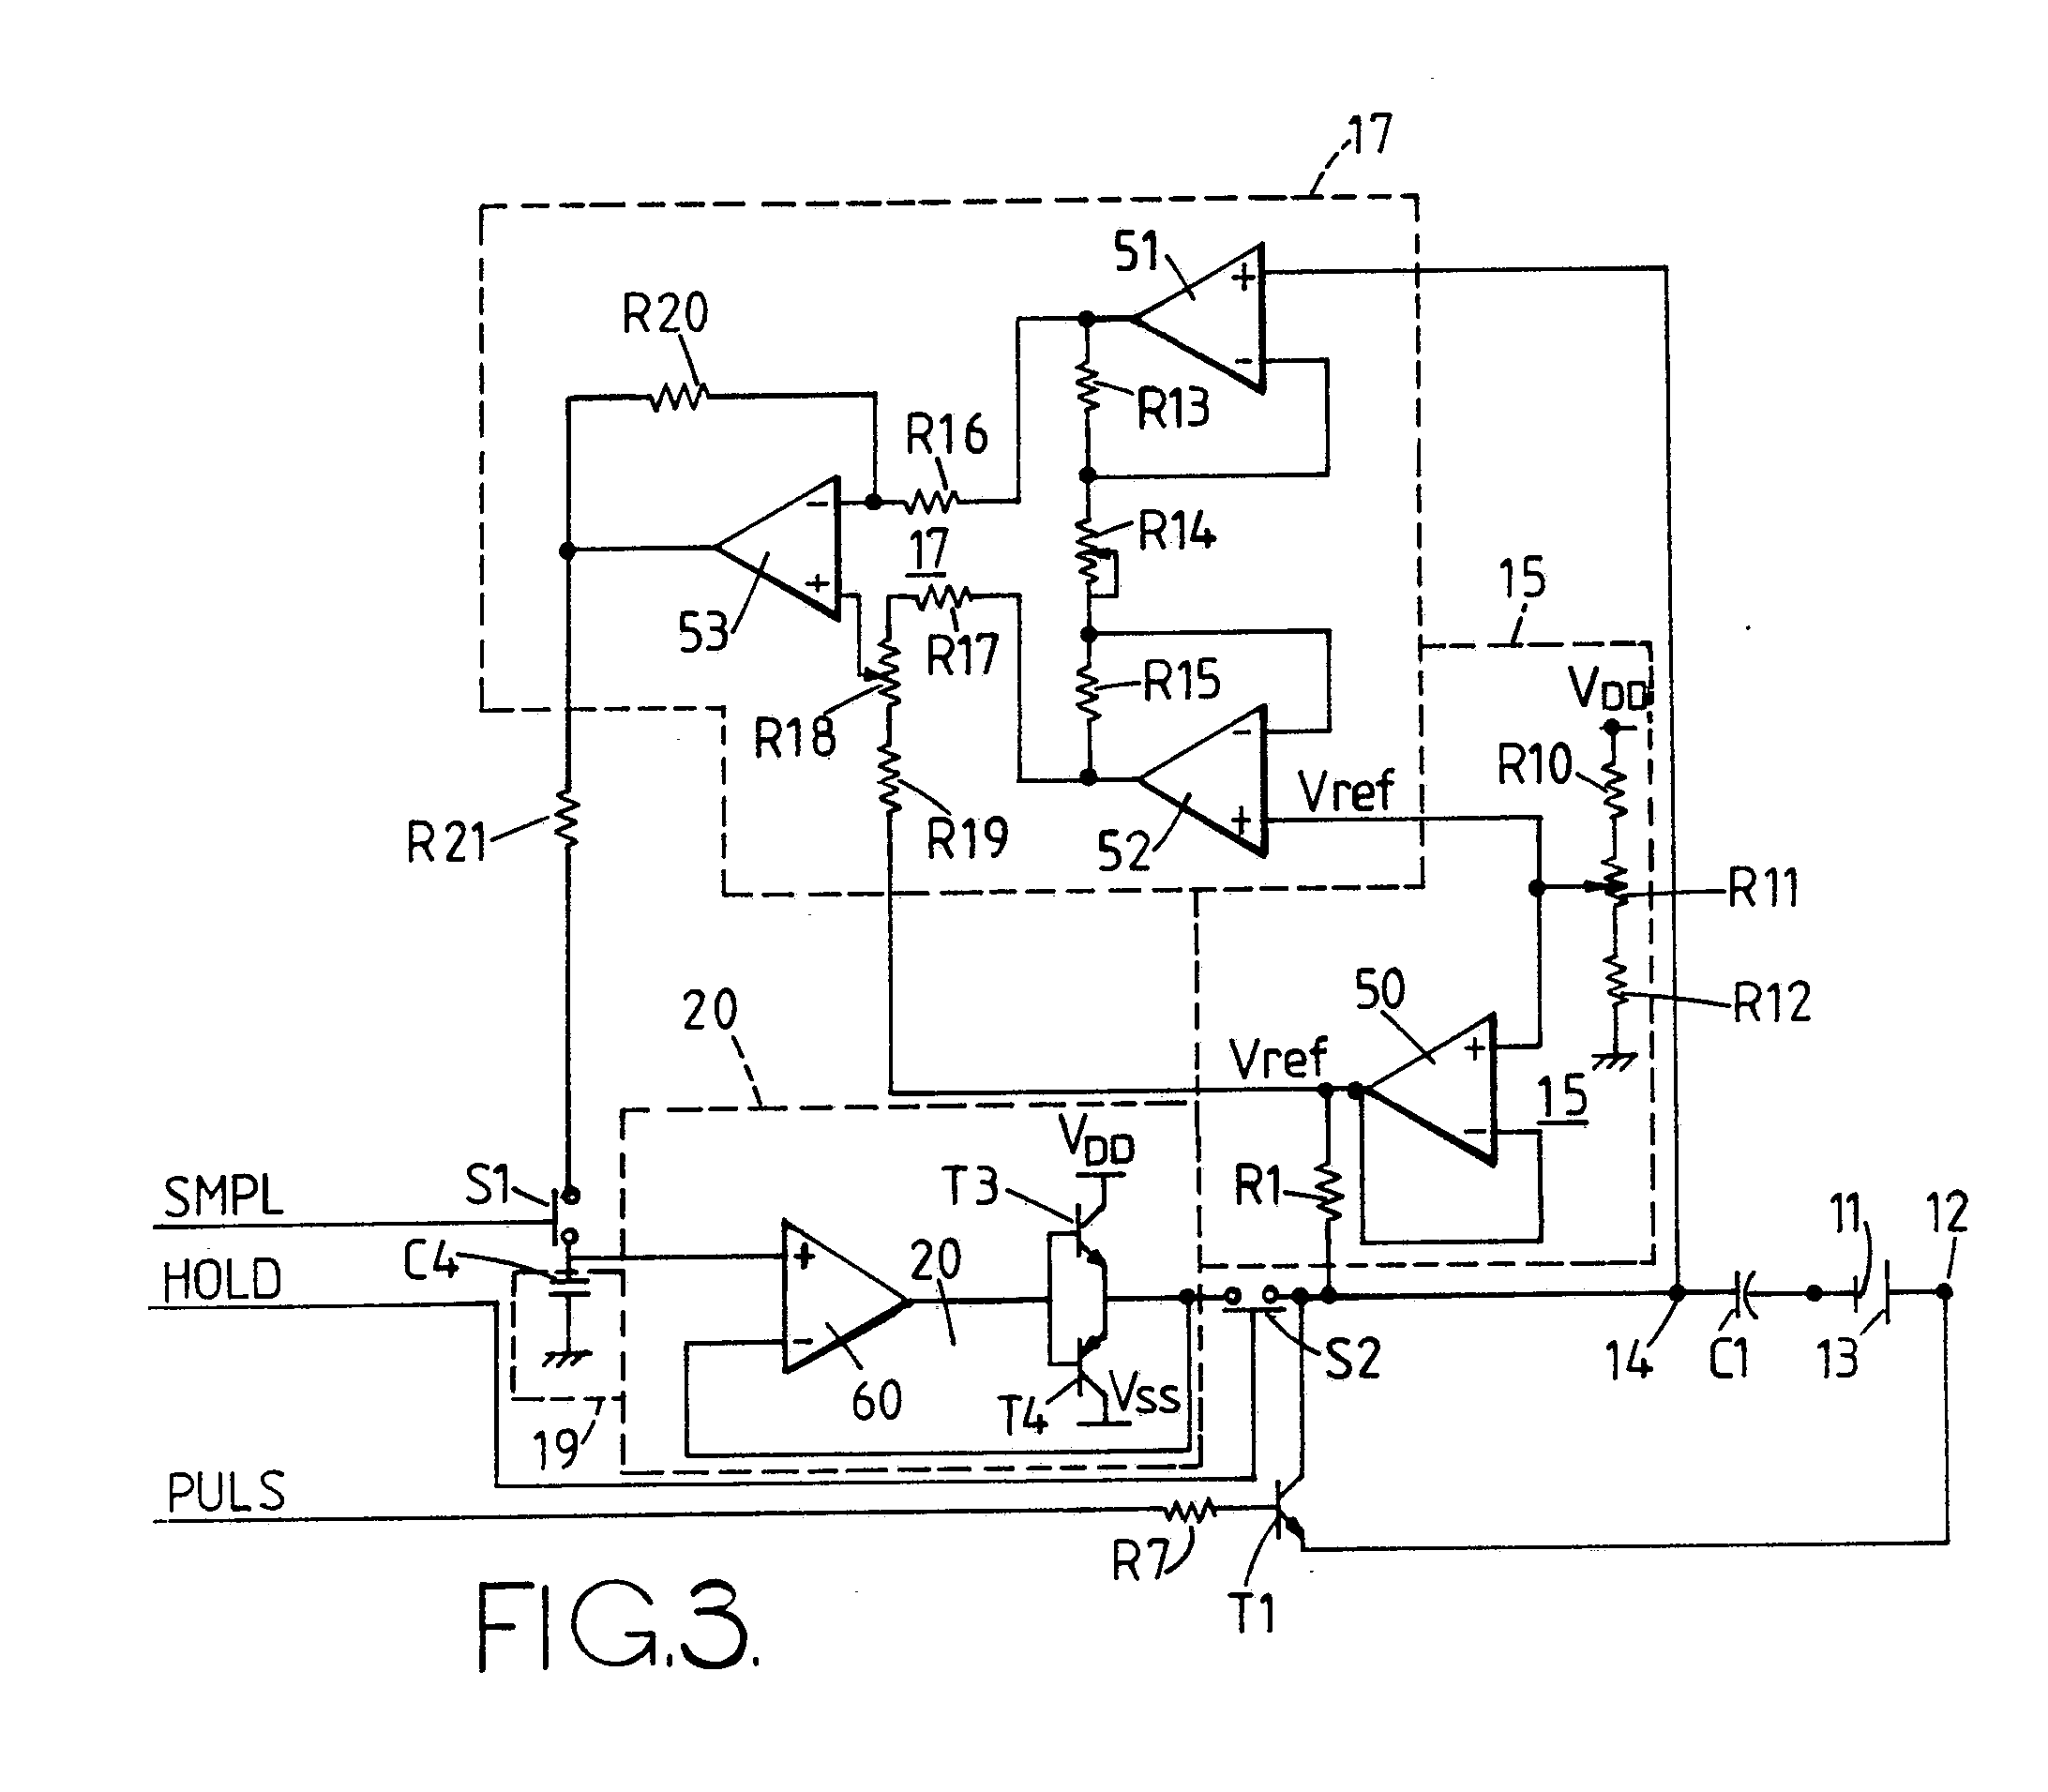
\includegraphics[width=9.9cm]{./bilder/PacemakerCircuit.png}
\end{textblock*}

\vissteduatt{Visste du att pacemakern är en Lundauppfinning?}


\newpage
\resetBackground

\subsection*{Mer jul} 
\index[alfa]{Mer jul}
\index[anfa]{Mer jul} 
\songinfo{Av: Adolphson \& Falk
}

\begin{parse lines}[\noindent]{#1\\}
    Jag är en lugn person med takt och ton
    måttfull och balanserad
    Jag är tyst och still och det ska mycket till 
    innan jag blir exalterad
    Men jag har en last som håller mig fast 
    i ett järngrepp varje vinter
    När året är slut och snön ligger djup 
    och slädarnas medar slinter

    Jag vill ha mer jul
    Ge mig mer jul
    Jag vill ha mer jul
    Ge mig mer jul
    Tusen stjärnor som tindrar,
    glitter så långt jag ser
    Av juleljus som glimmar,
    vill jag ha mer

    En show glöms bort om den bara visar opp 
    effekter som man knappast anar
    Så ge mig trettio grader kallt, tomtar överallt 
    och en skog av gröna granar
    Jag vill ha snötyngda hus, tusentals ljus, 
    kulörta kulor i drivor
    Bjällerklang som ackompanjemang 
    på alla julens skivor    
\end{parse lines}

\newpage

\begin{parse lines}[\noindent]{#1\\}

    Jag vill ha mer jul…

    Ge mig en svårknäckt nöt, sötare gröt, 
    djupare dopp i grytan
    Glittrigare glim och grötigare rim 
    och mer Arne Weise i rutan
    Jag vill ha rymligare säck, segare knäck, 
    fetare fläsk från grisen
    Krimsigare krams, längre långdans 
    och raskare räv på isen

    Jag vill ha mer jul…

    Jag vill ha mer, mer
    Ge mig mer, mer
    Jag vill ha mer, mer
    Ge mig mer, mer

\end{parse lines}

\vissteduatt{Visste du att Mer jul spelas årligen i Edekvata oavbrutet från och \\med Glöggillet fram tills Julgillet är hållet?}

\newpage

\subsection*{Jag en liten nolla} 
\index[alfa]{Jag en liten nolla}
\index[anfa]{Jag en liten nolla}
\songinfo{Mel: Jag är fattig bonddräng\\
Text: Jan-Olof Sivtoft, E94}

\begin{parse lines}[\noindent]{#1\\}
    Jag, en liten nolla, på Elektro jag går
    Dagar går och kommer, medan jag pluggar på
    Labbar, löddar, räknar, programmerar och lär, 
    Går på föreläsning, inför tentan jag svär

    Jag en fattig nolla, pasta lever jag på
    Och när fredan kommer till Edekvata jag gå
    Sen, när jag blitt livad, vill jag dansa, umgås
    Vila hos en flicka, vill jag också förstås

    Sen så kommer helgen, och då vill CSN
    Att jag pluggar satan, men då festar jag än
    40 timmars vecka, gäller inte för oss
    För oss teknologer, e de dubbelt förstås

    Så går hela veckan, varje läsperiod
    Åren går och kommer, men jag är vid gott mod
    Jag tar mina tentor, samlar på mig poäng, 
    Jag tar min examen, sen så blir jag utslängd

    Nu så väntar livet, som civilingenjör
    Nu så ska jag skörda, tjäna pengar som smör
    Men man jobbar sliter, si så där 40 år
    Till barn, familj o staten, alla pengarna går
\end{parse lines}

\newpage

\begin{parse lines}[\noindent]{#1\\}
    Så när dagen kommer, invid himmelens port, 
    Lite rädd och lessen, för de synder jag gjort
    Inte skattefuska, köra fort, supa loss
    Herren Gud i himlen, är väl missnöjd förstås

    Jag, vid pärleporten, blir nu eftertänksam
    De allra bästa åren, alltför snabbt de försvann
    Hade allt för bråttom, bort från de som var bäst
    Åren på Elektro, saknar jag allra mest

    Men då säger Herren: (civil) ingenjören, kom hit! 
    Jag har sett din strävan, och ditt eviga slit
    Därför, ingenjören, är du välkommen här
    Himmelens Elektro till du antagen är

    Jag som liten ängel, står så still inför Gud, 
    och sen klär han på mej en Elektrovit skrud
    Nu du, säger Herren, börjar vi om igen 
    Nu du, liten nolla, nu har du kommit hem

    Till dig liten nolla, sensmoralen den är
    Ha ej allt för bråttom, under tiden du lär
    Tids nog får du jobba, resten utav ditt liv
    Därför ta till vara, på studentlivets tid
\end{parse lines}

\vissteduatt{Visste du att denna sjunges bäst på nollEgasque?}


\newpage